% (c) 2012 -2014 Dimitrios Vrettos - d.vrettos@gmail.com
\chapter{Insiemi}
\section{Insiemi ed elementi}

In matematica usiamo la parola \textit{insieme} per indicare un
raggruppamento, una collezione, una raccolta di oggetti, individui,
simboli, numeri, figure che sono detti \textit{elementi}
dell'insieme e che sono ben definiti e distinti tra di
loro.

La nozione di insieme e quella di elemento di un insieme in matematica
sono considerate nozioni primitive, nozioni che si preferisce non
definire mediante altre più semplici.

\begin{exrig}
 \begin{esempio}
 Sono insiemi:
 \begin{enumeratea}
  \item l'insieme delle lettere della parola RUOTA;
  \item l'insieme delle canzoni che ho ascoltato la settimana scorsa;
  \item l'insieme delle città della Puglia con più di~$\np{15000}$ abitanti;
  \item l'insieme delle lettere dell'alfabeto italiano;
  \item l'insieme dei numeri~1, 2, 3, 4, 5;
  \item l'insieme delle montagne d'Italia più alte di~$\np{1000}$ metri.
 \end{enumeratea}
 \end{esempio}
\end{exrig}

Per poter assegnare un insieme occorre soddisfare le seguenti condizioni:

\begin{itemize*}
\item bisogna poter stabilire con certezza e oggettività se un oggetto
è o non è un elemento dell'insieme;
\item gli elementi di uno stesso insieme devono essere differenti tra
loro, cioè un elemento non può essere ripetuto più volte nello stesso insieme.
\end{itemize*}

Non possono essere considerati insiemi:
\begin{itemize*}
 \item i film interessanti (non c'è un criterio oggettivo per stabilire se un film è interessante oppure no, uno stesso film
può risultare interessante per alcune persone e non interessante per altre);
 \item le ragazze simpatiche di una classe (non possiamo stabilire in maniera oggettiva se una ragazza è simpatica);
 \item le montagne più alte d'Italia (non possiamo dire se una montagna è tra le più alte poiché non è fissata
un'altezza limite);
 \item l'insieme delle grandi città d'Europa (non c'è un criterio per
stabilire se una città è grande);
\end{itemize*}

\ovalbox{\risolvi \ref{ese:5.1}}\vspazio


In generale, gli insiemi si indicano con lettere maiuscole~$A$, $B$, $C$, \ldots e
gli elementi con lettere minuscole~$a$, $b$, $c$, \ldots

Se un elemento~$a$ sta nell'insieme~$A$ si scrive~$a\in A$ e si legge ``$a$ appartiene ad~$A$''.
Il simbolo ``$\in$'' si chiama simbolo di \textit{appartenenza}.

Se un elemento~$b$ non sta nell'insieme~$A$ si scrive~$b\notin A$ e
si legge ``$b$ non appartiene ad~$A$''. Il simbolo ``$\notin$''
si chiama simbolo di \textit{non appartenenza}.

Il criterio che stabilisce se un elemento appartiene a un insieme si chiama \textit{proprietà caratteristica} dell'insieme.

Un altro modo per definire un insieme, oltre a quello di indicare la sua proprietà caratteristica, è quello di elencare i suoi elementi separati da virgole e racchiusi tra parentesi graffe. Ad esempio: $A=\{a\text{, }b\text{, }c\text{, }d\}$.

Per indicare alcuni insiemi specifici vengono utilizzati simboli particolari:
\begin{itemize*}
 \item $\insN$ si utilizza per indicare l'insieme dei numeri naturali:~$\insN=\{0\text{, }1\text{, }2\text{, }3\text{, }\ldots\}$;
 \item $\insZ$ si utilizza per indicare i numeri interi relativi:~$\insZ=\{\ldots\text{, }-2\text{, }-1\text{, }0\text{, }+1\text{, }+2\text{, }\ldots\}$;
 \item $\insQ$ si utilizza per indicare i numeri razionali:~$\insQ=\{\dfrac{1}{2}\text{, }-\dfrac{3}{5}\text{, }\dfrac{5}{1}\text{, }-\dfrac{4}{17}\text{, }\np{12,34}\text{, }8\text{, }\np{0,}\overline{25}\text{, }\ldots\}$.
 \end{itemize*}


 \begin{exrig}
 \begin{esempio}
Indica con il simbolo opportuno quali dei seguenti elementi appartengono
o non appartengono all'insieme $A$ dei giorni della
settimana: lunedì, martedì, gennaio, giovedì, dicembre, estate.

Gennaio e dicembre sono mesi dell'anno, perciò scriviamo:
\[\text{lunedì}\in A\text{,~~~}\text{martedì}\in A\text{,~~~}\text{gennaio}\notin A\text{,~~~}\text{giovedì}\in A\text{,~~~}\text{dicembre}\notin A\text{,~~~}\text{estate}\notin A.\]
 \end{esempio}
\end{exrig}

Consideriamo l'insieme~$A=\{\text{r, s, t}\}$ e l'insieme~$B$ delle consonanti della parola
``risate''. Possiamo osservare che~$A$ e~$B$ sono due insiemi costituiti dagli stessi
elementi; diremo che sono \textit{insiemi uguali}.

\begin{definizione}
 Due insiemi~$A$ e~$B$ si dicono \emph{uguali} se sono formati dagli stessi elementi, anche se
disposti in ordine diverso. In simboli si scrive~$A=B$. Altrimenti i due insiemi si dicono \emph{diversi}, in simboli~$A\neq B$.
\end{definizione}

\ovalbox{\risolvii \ref{ese:5.2}, \ref{ese:5.3}, \ref{ese:5.4}, \ref{ese:5.5}, \ref{ese:5.6}, \ref{ese:5.7}, \ref{ese:5.8}}

\section{Insieme vuoto, insieme universo, cardinalità}\label{sect:universo}

Consideriamo l'insieme~$A=\{\text{consonanti della parola ``AIA''}\}$. Poiché la parola ``AIA'' non
contiene consonanti, l'insieme~$A$ è privo di elementi.

\begin{definizione}
 Un insieme privo di elementi si chiama \emph{insieme vuoto} e lo si indica con il simbolo~$\emptyset$ o $\{ \}$.
\end{definizione}

\osservazione $\{ \}=\emptyset$ ma~$\{\emptyset \}\neq\emptyset$ dato che la scrittura~$\{\emptyset \}$ rappresenta un insieme che ha come unico elemento l'insieme vuoto, quindi non è vuoto.
\pagebreak
\begin{exrig}
 \begin{esempio}
 Alcuni insiemi vuoti.
 \begin{enumeratea}
  \spazielenx
\item L'insieme dei numeri negativi maggiori di~5 è vuoto;
\item l'insieme delle capitali europee con meno di~50 abitanti è vuoto;
\item l'insieme dei numeri naturali minori di~0 è vuoto.
 \end{enumeratea}
 \end{esempio}
\end{exrig}

La frase <<l'insieme degli studenti che vengono a scuola con il motorino>> non definisce un
insieme particolare. Occorre definire il contesto, l'ambiente che fa individuare gli elementi
dell'insieme. Se l'ambiente è la classe~1\textsuperscript{a}C gli elementi considerati saranno certamente diversi, e probabilmente meno numerosi, di quelli che compongono l'ambiente di un'intera scuola o di un'intera
città. Quando si identifica un insieme, occorre indicare anche l'ambiente di riferimento da cui trarre gli elementi che appartengono al nostro insieme. Questo insieme si chiama \emph{insieme universo} e rappresenta il contesto, l'ambiente su cui faremo le nostre osservazioni. In generale l'insieme universo per un insieme~$A$ è semplicemente un insieme che contiene~$A$. Solitamente l'insieme universo viene indicato con~$U$.

\subsection{Cardinalità}

\begin{definizione}
 Si definisce \emph{cardinalità} (o \emph{potenza}) di un insieme finito il numero
degli elementi dell'insieme. Essa viene indicata con uno dei seguenti simboli~$\valass{A}$, \#($A$) o~$\card(A)$.
\end{definizione}

Per poter parlare di cardinalità di un insieme qualsiasi, che
comprenda anche insiemi infiniti come gli insiemi numerici, occorre una
definizione più complessa che qui non daremo.

\begin{exrig}
 \begin{esempio}
 Esempi di cardinalità.
 \begin{enumeratea}
  \item L'insieme~$A$ delle vocali dell'alfabeto italiano ha~5 elementi, quindi~$\card(A)=5$;
  \item l'insieme~$B$ dei multipli di~3 minori di~10 ha~3 elementi, quindi~$\card(B)=3$.
 \end{enumeratea}
 \end{esempio}
\end{exrig}

\ovalbox{\risolvii \ref{ese:5.9}, \ref{ese:5.10}, \ref{ese:5.11}, \ref{ese:5.12}, \ref{ese:5.13}, \ref{ese:5.14}}

\section{Rappresentazione degli insiemi}

Esistono diversi modi per rappresentare un insieme e quindi per indicare
con precisione i suoi elementi.

\subsection{Rappresentazione tabulare}

La rappresentazione tabulare è la descrizione più elementare di un
insieme; consiste nell'elencare tutti gli elementi dell'insieme separati da virgole e racchiusi tra le
parentesi graffe.

Per esempio, definiamo un insieme~$X$ con la scrittura:~$X=\{\text{1, 2, 3, 5}\}$.
Non è importante l'ordine in cui vengono scritti gli elementi, cioè
\[X=\{\text{1, 2, 3, 5}\}=\{\text{2, 1, 5, 3}\}.\]

È invece necessario che ogni elemento dell'insieme compaia una sola volta. Ad esempio, per rappresentare
l'insieme~$Y$ delle lettere della parola ``autunno'', scriviamo
\[Y = \{\text{a, u, t, n, o}\}.\]

Si può utilizzare questa rappresentazione anche per insiemi numerosi e addirittura infiniti. In questi casi si elencano i primi elementi
dell'insieme e in fondo all'elenco si mettono tre punti di sospensione lasciando intendere come continuare la serie.

Per esempio, l'insieme dei multipli di~3 si può indicare con la seguente rappresentazione tabulare:
\[X=\{\text{0, 3, 6, 9, 12, 15, 18, 21, }\ldots\}.\]


\begin{exrig}
 \begin{esempio}
Rappresentazione degli insiemi:
 \begin{enumeratea}
\item l'insieme~$G$ dei primi~3 giorni della settimana si indica:~$G=\{\text{lunedì, martedì, mercoledì}\}$;
\item l'insieme~$A$ delle lettere della parola ``associazione'' si indica:~$A=\{\text{a, s, o, c, i, z, n, e}\}$.
\end{enumeratea}
 \end{esempio}
\end{exrig}

\ovalbox{\risolvii \ref{ese:5.15}, \ref{ese:5.16}, \ref{ese:5.17}, \ref{ese:5.18}}

\subsection{Rappresentazione per proprietà caratteristica}

Per quegli insiemi i cui elementi soddisfano una certa proprietà che
li caratterizza, possiamo usare proprio questa proprietà per
descrivere più sinteticamente l'insieme che li contiene.

Per esempio, l'insieme~$Y$ dei divisori di~10 può essere definito come: \[Y=\{x\mid x \text{ è un divisore di }10\}\]
e si legge ``$Y$ è l'insieme degli elementi~$x$ tali che~$x$ è un divisore di~10''.

In questa scrittura si mette in evidenza la caratteristica degli elementi dell'insieme.
La rappresentazione tabulare dello stesso insieme è~$Y=\{\text{1, 2, 5, 10}\}$. L'espressione ``tale che'', che è stata rappresentata per mezzo del simbolo ``$|$'', può essere indicata anche per mezzo del simbolo ``:''.

La rappresentazione per caratteristica dell'insieme~$X$
dei naturali minori di~15 è: \[X=\{x\in\insN\mid x<15\}\]
e si legge ``$X$ è l'insieme dei numeri naturali~$x$ tali che~$x$ è minore di~15''.

L'insieme che viene indicato nella prima parte della rappresentazione (nell'ultimo esempio è
l'insieme dei numeri naturali~$\insN$) è l'\textit{insieme universo} (sezione \ref{sect:universo}) al quale si fa riferimento.
Questo metodo è particolarmente utile quando l'insieme da rappresentare contiene molti elementi.

\begin{exrig}
 \begin{esempio}
 Esempi di definizioni di insiemi per mezzo della loro proprietà caratteristica:
 \begin{enumeratea}
\item l'insieme~$A$ delle rette incidenti a una retta~$t$ assegnata si può rappresentare come:
\[A=\{r\mid r\text{ è una retta incidente a } t\}\]
\item l'insieme~$B$ dei numeri naturali maggiori di~100 può essere rappresentato come:
\[B=\{n\in\insN\mid n>100\}\]
\item l'insieme~$P$ dei numeri pari può essere rappresentato come:
\[P=\{n\in\insN\mid n=2\cdot m\text{, con }m\in\insN\}\]
\item l'insieme~$C$ dei numeri interi relativi compresi tra~$-10$ e~$+100$, estremi inclusi:
\[C=\{n\in\insZ\mid -10\le n\le 100\}.\]
\end{enumeratea}
 \end{esempio}
\end{exrig}

\ovalbox{\risolvii \ref{ese:5.19}, \ref{ese:5.20}, \ref{ese:5.21}, \ref{ese:5.22}, \ref{ese:5.23}, \ref{ese:5.24}, \ref{ese:5.25}, \ref{ese:5.26}, \ref{ese:5.27}, \ref{ese:5.28}, \ref{ese:5.29},\ref{ese:5.30}, \ref{ese:5.31},}

\vspazio\ovalbox{\ref{ese:5.32}}

\subsection{Rappresentazione grafica (Diagramma di Eulero-Venn)}

In questa rappresentazione grafica, detta anche \textit{rappresentazione
di Eulero-Venn}\footnote{in onore del matematico svizzero Leonhard Euler, noto in Italia come Eulero, (1707 - 1783) e del matematico e statistico inglese John Venn (1834 - 1923).} si disegna una linea chiusa all'interno della quale gli elementi
dell'insieme si indicano con dei punti. Solitamente si scrive all'esterno il nome dell'insieme
e vicino ad ogni punto il valore ad esso associato.

\begin{exrig}
 \begin{esempio}
 $A$ è l'insieme dei numeri naturali minori di~6, cioè $A=\{\text{0, 1, 2, 3, 4, 5}\}$.
 La sua rappresentazione con un diagramma di Eulero-Venn è la seguente
 \begin{center}
  % (c) 2012 Dimitrios Vrettos - d.vrettos@gmail.com
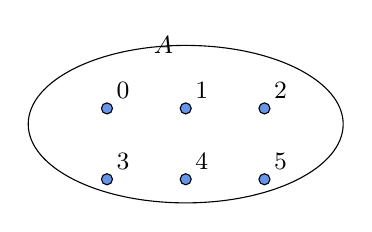
\begin{tikzpicture}[x=2cm,font=\small]
\draw (0,0)circle (1) (0,1) node[ left=1] {$A$};
\begin{scope}[fill=CornflowerBlue, draw=black]
\foreach \x/\xtext in {-.5/0,0/1,.5/2}
\filldraw (\x,.2) circle (2pt) node[above right] {\xtext};
\foreach \y/\ytext in {-.5/3,0/4,.5/5}{
\filldraw (\y,-.7) circle (2pt) node[above right] {\ytext};
}
\end{scope}
\end{tikzpicture}

 \end{center}

 \end{esempio}

 \begin{esempio}
 $B$ è l'insieme delle lettere della parola ``TARTARUGA'', $B=\{\text{t, a, r, u, g}\}$.
 La sua rappresentazione con un diagramma di Eulero-Venn è la seguente
 \begin{center}
  % (c) 2012 Dimitrios Vrettos - d.vrettos@gmail.com
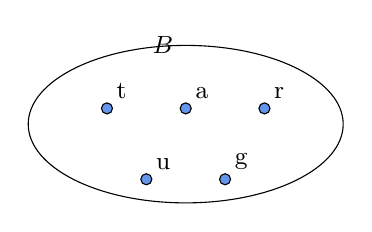
\begin{tikzpicture}[x=2cm,font=\small]
\draw (0,0)circle (1) (0,1) node[ left=1] {$B$};
\begin{scope}[fill=CornflowerBlue, draw=black]
\foreach \x/\xtext in {-.5/t,0/a,.5/r}
\filldraw (\x,.2) circle (2pt) node[above right] {\xtext};
\foreach \y/\ytext in {-.25/u,.25/g}{
\filldraw (\y,-.7) circle (2pt) node[above right] {\ytext};
}
\end{scope}
\end{tikzpicture}

 \end{center}

 \end{esempio}

\end{exrig}

Un insieme può essere rappresentato con una qualsiasi delle
rappresentazioni indicate. Se un insieme è infinito o è costituito
da un numero elevato di elementi la rappresentazione più pratica è
quella per caratteristica.
\pagebreak
\begin{exrig}
 \begin{esempio}
 Rappresentare l'insieme~$C$ dei multipli di~5.

 Per caratteristica:~$C=\{n\in\insN\mid n\text{ è multiplo di }5\}$ oppure
$C=\{n\in\insN\mid n=5\cdot m$, $m\in\insN\}$

Tabulare:~$C=\{\text{0, 5, 10, 15, 20, 25, 30, 35, }\dots\}$. I puntini di sospensione indicano che l'elenco continua.

Rappresentazione con diagramma di Eulero-Venn:
\begin{center}
 % (c) 2012 Dimitrios Vrettos - d.vrettos@gmail.com
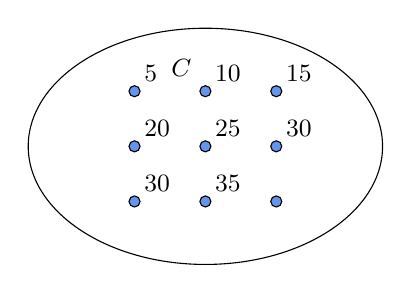
\begin{tikzpicture}[x=1.5cm,font=\small]
    \draw (0,0)circle (1.5) (0,1) node[ left=1.5] {$C$};
    \begin{scope}[fill=CornflowerBlue, draw=black]
\foreach \x/\xtext in {-.6/5,0/10,.6/15}
\filldraw (\x,.7) circle (2pt) node[above right] {\xtext};
\foreach \y/\ytext in {-.6/20,0/25,.6/30}
\filldraw (\y,0) circle (2pt) node[above right] {\ytext};
\foreach \z/\ztext in {-.6/30,0/35,.6/{}}
\filldraw(\z,-.7) circle (2pt) node [above right]  {\ztext};
\end{scope}
\end{tikzpicture}

\end{center}
 \end{esempio}
\end{exrig}

\ovalbox{\risolvii \ref{ese:5.33}, \ref{ese:5.34}, \ref{ese:5.35}, \ref{ese:5.36}, \ref{ese:5.37}, \ref{ese:5.38}, \ref{ese:5.39}, \ref{ese:5.40}}

\section{Sottoinsieme}

Consideriamo l'insieme~$A$ degli abitanti di Milano e l'insieme~$B$ degli abitanti di Milano
con età superiore ai~40 anni. Gli abitanti ultra quarantenni di Milano fanno parte della popolazione di Milano, cioè tutti gli
elementi dell'insieme~$B$ sono anche elementi di~$A$: si dice che~$B$ è sottoinsieme di~$A$ e si scrive~$B\subseteq A$.

\begin{definizione}
Dati due insiemi~$X$ e~$Y$, si dice che~$Y$ è un \emph{sottoinsieme} di~$X$
se ogni elemento di~$Y$ è anche elemento di~$X$.
In simboli:~$Y\subseteq X$, che si legge
``$Y$ è incluso in~$X$'' o ``$Y$ è sottoinsieme di~$X$''.
\end{definizione}

La rappresentazione con un diagramma di Eulero-Venn è la seguente:
\begin{center}
\input{./lbr/chap05/fig005_Venn.pgf}
\end{center}
Se~$a$ è un elemento del sottoinsieme~$Y$, allora lo sarà anche dell'insieme~$X$:
\begin{center}
se~$a\in Y$ e~$Y\subseteq X$, allora~$a\in X$\qquad oppure \qquad $a\in Y$ e~$Y\subseteq X \:\Rightarrow\:a\in X$.
\end{center}

Dalla stessa definizione, si deduce che ogni insieme è sottoinsieme di
se stesso, in simboli~$X\subseteq X$.

Nel caso in cui tutti gli elementi di~$Y$ siano elementi di~$X$ e tutti gli elementi di~$X$ siano elementi di
$Y$ si ha che~$X=Y$, e~$Y$ si dice \emph{sottoinsieme improprio} di~$X$.
Se~$X\subseteq Y$ e~$Y\subseteq X$, allora~$Y=X$.

Tra i sottoinsiemi di un insieme si considera anche
l'insieme vuoto. Cioè, qualunque sia
l'insieme~$X$ risulta~$\emptyset \subseteq X$.
Quindi l'insieme vuoto è considerato un sottoinsieme improprio di qualunque insieme.

Se~$Y$ è un sottoinsieme non vuoto di~$X$ e~$X$ ha altri elementi oltre a quelli di~$Y$
si dice che~$Y$ è un \emph{sottoinsieme proprio} di~$X$ e si scrive~$Y\subset X$.

La scrittura~$Y\subseteq X$ si usa quando non si sa in modo certo se~$Y=X$ o meno.

\begin{exrig}

\begin{esempio}
Consideriamo l'insieme~$X=\{$lettere della parola ``autunno''$\}$ e
l'insieme~$Y=\{$lettere della parola ``notaio''$\}$; possiamo affermare che ogni
elemento di~$Y$ è anche elemento di~$X$? La risposta è negativa, infatti~$\text{i}\in Y$ ma
$\text{i}\notin X$ quindi~$Y$ non è sottoinsieme di~$X$ e si scrive~$Y\not\subset X$.
\end{esempio}

\begin{esempio}
Sia~$A$ l'insieme delle lettere dell'alfabeto italiano e~$V$
l'insieme delle vocali, allora si può scrivere
$V\subset A$; cioè~$V$ è un sottoinsieme proprio di~$A$,
come si può anche vedere dalla rappresentazione grafica.
\begin{center}
 % (c) 2012 Dimitrios Vrettos - d.vrettos@gmail.com
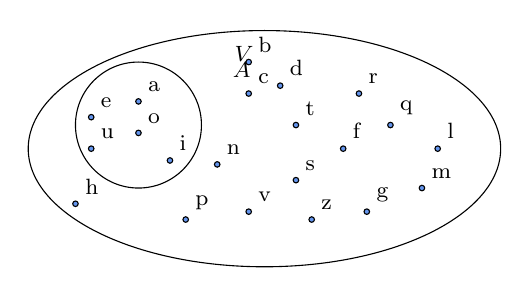
\begin{tikzpicture}[x=2cm,font=\footnotesize, fill=CornflowerBlue]
    \draw (0,0)circle (1.5) (0,1) node[ left=1.5] {$A$};
\filldraw (-.8,.6) circle (1pt) node[above right] {a};
\filldraw (-1.1,.4) circle (1pt) node[above right] {e};
\filldraw (-.6,-.15) circle (1pt) node[above right] {i};
\filldraw (-.8,.2) circle (1pt) node[above right] {o};
\filldraw (-1.1,0) circle (1pt) node[above right] {u};

\filldraw (-.1,1.1) circle (1pt) node[above right] {b};
\filldraw (-.1,.7) circle (1pt) node[above right] {c};
\filldraw (.1,.8) circle (1pt) node[above right] {d};
\filldraw (.5,0) circle (1pt) node[above right] {f};
\filldraw (.65,-.8) circle (1pt) node[above right] {g};
\filldraw (-1.2,-.7) circle (1pt) node[above right] {h};
\filldraw (1.1,0) circle (1pt) node[above right] {l};
\filldraw (1,-.5) circle (1pt) node[above right] {m};
\filldraw (-.3,-.2) circle (1pt) node[above right] {n};
\filldraw (-.5,-.9) circle (1pt) node[above right] {p};
\filldraw (.8,.3) circle (1pt) node[above right] {q};
\filldraw (.6,.7) circle (1pt) node[above right] {r};
\filldraw (.2,-.4) circle (1pt) node[above right] {s};
\filldraw (.2,.3) circle (1pt) node[above right] {t};
\filldraw (-.1,-.8) circle (1pt) node[above right] {v};
\filldraw (.3,-.9) circle (1pt) node[above right] {z};
 \begin{scope}[y=2cm]]
     \draw (-.8,.15)circle (.4) (0,.6) node[left=.4] {$V$};
 \end{scope}
\end{tikzpicture}

\end{center}
\end{esempio}

\begin{esempio}
Sia~$C=\{1\}$, allora~$C$ non ha sottoinsiemi propri;
mentre i suoi sottoinsiemi impropri sono~$C=\{1\}$ e
l'insieme vuoto~$\emptyset $.
\end{esempio}

\begin{esempio}
Sia~$A$ l'insieme delle auto esposte in un
autosalone e~$U$ l'insieme delle auto usate
esposte nello stesso autosalone. Si ha che~$U$ è un
sottoinsieme di~$A$, ma senza avere ulteriori informazioni non
possiamo escludere che tutte le auto esposte siano usate, dobbiamo
perciò scrivere~$U\subseteq A$. Se invece sappiamo che nessuna
auto esposta è usata, allora~$U=\emptyset $.
\end{esempio}
\end{exrig}

\ovalbox{\risolvii \ref{ese:5.41}, \ref{ese:5.42}, \ref{ese:5.43}, \ref{ese:5.44}, \ref{ese:5.45}, \ref{ese:5.46}}

\section{Insieme delle parti}

Consideriamo l'insieme~$A$ dei numeri naturali
compresi tra~0 e~100. A partire da questo insieme possiamo formare
gruppi costituiti dai soli numeri multipli di~10, dai numeri pari, da
quelli dispari, da quelli divisibili per~7 e così via. Quindi con gli
elementi dell'insieme~$A$ possiamo formare molti
altri insiemi che sono sottoinsiemi di~$A$.

\begin{exrig}
 \begin{esempio}
Determinare tutti i sottoinsiemi di~$A=\{$1, 2, 3$\}$.

$\emptyset \subseteq A$, infatti l'insieme vuoto è un
sottoinsieme improprio di qualunque insieme.

Elenchiamo tutti i sottoinsiemi costituiti da un solo elemento: $\{1\}$, $\{2\}$, $\{3\}$.
Elenchiamo ora tutti i sottoinsiemi costituiti da due elementi: $\{$1, 2$\}$, $\{$1, 3$\}$, $\{$2, 3$\}$.
L'unico sottoinsieme costituito da tre elementi è~$A$ stesso, possiamo scrivere:
$\{$1, 2, 3$\}\subseteq A$. In tutto si hanno 8 sottoinsiemi.
 \end{esempio}

\end{exrig}

\begin{definizione}
Dato un insieme~$A$, si chiama \emph{insieme delle parti} o (\emph{insieme potenza}) di~$A$ l'insieme $\wp(A)$ che ha come elementi
tutti i sottoinsiemi propri ed impropri di~$A$.
\end{definizione}

L'insieme delle parti di un insieme $A$ ha sempre come
elementi~$\emptyset $ e~$A$, quindi~$\emptyset\in\wp (A)$ e
$A\in\wp (A)$.
Il numero degli elementi di~$\wp (A)$, cioè dei suoi possibili
sottoinsiemi, propri e impropri, dipende dal numero degli elementi di~$A$.

\begin{exrig}
 \begin{esempio}
 L'insieme vuoto ha come unico sottoinsieme se stesso,
quindi~$\wp (\emptyset )=\{\emptyset \}$.
 \end{esempio}

\begin{esempio}
 Dato l'insieme~$A=\{a\}$, i suoi possibili sottoinsiemi
propri ed impropri sono:~$S_{1}=\emptyset$, $S_{2}=\{a\}$;
allora~$\wp (A)=\{S_{1}\text{, }S_{2}\}$.
 \end{esempio}

\begin{esempio}
 Dato l'insieme~$B=\{\text{matita, penna}\}$ i
suoi possibili sottoinsiemi propri ed impropri sono:~$S_{1}=\emptyset$,
$S_{2}=B=\{\text{matita, penna}\}$, $S_{3}=\{\text{matita}\}$,
$S_{4}=\{\text{penna}\}$;
allora~$\wp (A)=\{S_{1}\text{, }S_{2}\text{, }S_{3}\text{, }S_{4}\}$.
 \end{esempio}

\begin{esempio}
 Dato l'insieme~$B=\{\text{1, 2, 3}\}$, i suoi possibili
sottoinsiemi propri ed impropri sono:~$S_{1}=\emptyset$,
$S_{2}=B=\{\text{1, 2, 3}\}$, $S_{3}=\{1\}$, $S_{4}=\{2\}$, $S_{5}=\{3\}$,
$S_{6}=\{1\text{, }2\}$, $S_{7}=\{1\text{, }3\}$, $S_{8}=\{2\text{, }3\}$;
allora~$\wp (A)=\{S_{1}\text{, }S_{2}\text{, }S_{3}\text{, }S_{4}\text{, }S_{5}\text{, }S_{6}\text{, }S_{7}\text{, }S_{8}\}$.
 \end{esempio}
 \end{exrig}

 Riassumendo:
\begin{itemize*}
\item se~$A=\emptyset $ l'insieme delle parti ha~1 solo elemento;
\item se~$A$ ha~1 elemento allora l'insieme delle parti ha~2 elementi;
\item se~$A$ ha~2 elementi, l'insieme delle parti ne ha~4;
\item se~$A$ ha~3 elementi, l'insieme delle parti ne ha~8.
\end{itemize*}

Generalizzando, se~$A$ ha~$n$ elementi, l'insieme delle parti $\wp (A)$ ne ha~$2^{n}$.

\vspazio\ovalbox{\risolvii \ref{ese:5.47}, \ref{ese:5.48}, \ref{ese:5.49}, \ref{ese:5.50}, \ref{ese:5.51}}

\section{Insieme unione}

Prendiamo l'insieme~$P$ dei numeri pari e l'insieme~$D$ dei numeri dispari; allora
l'insieme~$\insN$ dei numeri naturali è dato dall'unione dei due insiemi~$P$ e~$D$.

\begin{definizione}
Dati due insiemi~$A$ e~$B$, si dice
\emph{insieme unione} l'insieme~$C$, composto da tutti gli elementi appartenenti ad
$A$ o a~$B$ o a entrambi.
In simboli:~$C=A\cup B$ e si legge ``$A$ unito a~$B$''
o ``$A$ unione~$B$''.
\end{definizione}
\begin{center}
 % (c) 2012 Dimitrios Vrettos - d.vrettos@gmail.com
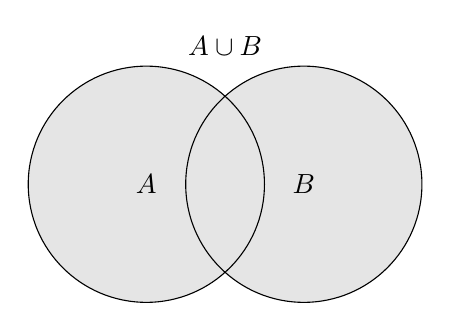
\begin{tikzpicture}[filled/.style={fill=circle area, draw=black, thin}]

\def\firstcircle{(0,0) circle (1.5cm)}
\def\secondcircle{(0:2cm) circle (1.5cm)}

\definecolor{circle area}{gray}{.9}

 \draw[filled] \firstcircle node {$A$}
                  \secondcircle node {$B$};
 \node[anchor=south] at (current bounding box.north) {$A \cup B$};
\end{tikzpicture}

\end{center}
Mediante la proprietà caratteristica si scrive:~$C=A\cup B=\{x\mid (x\in A)\text{ o }(x\in B)\}$.

\subsection{Proprietà dell'unione tra insiemi}

\begin{enumeratea}
\item $A\cup B=B\cup A$: proprietà \emph{commutativa} dell'unione;
\item $(A\cup B)\cup C=A\cup (B\cup C)$: proprietà \emph{associativa} dell'unione;
\item se~$B\subset A$, allora~$A\cup B=A$;
\item $A\cup \emptyset =A$;
\item $A\cup A=A$: proprietà di \emph{idempotenza} dell'unione;
\item $\emptyset \cup \emptyset = \emptyset $.
\end{enumeratea}

\begin{exrig}
 \begin{esempio}
Siano~$D=\{$1, 3, 5$\}$ e~$P=\{$2, 4, 6$\}$ allora \[N=P\cup D=\{1, 2, 3, 4, 5, 6\}.\]
\begin{center}
 \input{./lbr/chap05/fig008_unii.pgf}
\end{center}
\end{esempio}

\begin{esempio}
Siano~$X=\{$do, re, mi, fa, sol, la, si$\}$
e~$Y=\{$do, re, mi$\}$, allora, poiché $Y\subset X$, \[W=X\cup Y=X=\{\text{do, re, mi, fa, sol, la, si}\}.\]
\begin{center}
 \input{./lbr/chap05/fig009_uniii.pgf}
\end{center}
\end{esempio}
\end{exrig}

\ovalbox{\risolvii \ref{ese:5.52}, \ref{ese:5.53}, \ref{ese:5.54}, \ref{ese:5.55}}

\section{Insieme intersezione}

\begin{definizione}
Dati due insiemi~$A$ e~$B$, si dice \emph{insieme intersezione} di~$A$ e~$B$, l'insieme
$C$ composto da tutti gli elementi appartenenti contemporaneamente ad
$A$ e a~$B$, ossia comuni a entrambi.
In simboli:~$C=A\cap B$, che si legge
``$A$ intersecato a~$B$'' o ``$A$ intersezione~$B$''.
\end{definizione}

\begin{exrig}
 \begin{esempio}
Se~$A$ è l'insieme delle lettere della parola ``matematica'' e~$B$ è l'insieme delle lettere della parola
``materia''. Quali elementi di~$A$ stanno in~$B$? Quali elementi di~$B$ stanno in~$A$? Quali sono gli elementi
che stanno in entrambi gli insiemi?
\begin{itemize}
 \item L'insieme degli elementi di~$A$ che stanno in~$B$ è $\{$m, a, t, e, i$\}$;
 \item l'insieme degli elementi di~$B$ che stanno in~$A$ è $\{$m, a, t, e, i$\}$;
 \item l'insieme degli elementi che stanno sia in~$A$ sia in~$B$ è $\{$m, a, t, e, i$\}$.
\end{itemize}
\end{esempio}
\end{exrig}
\begin{center}
 \input{./lbr/chap05/fig011_inter.pgf}
\end{center}
Mediante proprietà caratteristica si scrive:~$C=A\cap B=\{x\mid (x\in A)\text{ e }(x\in B)\}$.

\begin{definizione}
Dati due insiemi~$A$ e~$B$, essi si dicono \emph{disgiunti} se non hanno elementi in comune, ossia se la loro intersezione è vuota. In simboli~$A \cap B = \emptyset$.
\end{definizione}

\begin{exrig}
 \begin{esempio}
Siano~$D=\{\text{1, 3, 5}\}$ e~$P=\{\text{2, 4, 6}\}$ allora~$N=P\cap D=\emptyset$. Gli insiemi $P$ e $D$ sono disgiunti.
\begin{center}
 % (c) 2012 Dimitrios Vrettos - d.vrettos@gmail.com
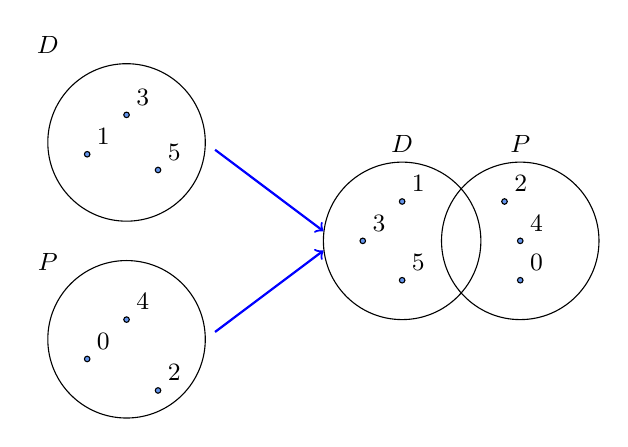
\begin{tikzpicture}[font=\small, fill=CornflowerBlue]
\draw (0,1.25)circle (1) (-1,2.25) node[above] {$D$};
\draw(0,-1.25) circle (1) (-1,-.5) node [above]  {$P$};
\draw (3.5,0) circle (1) (3.5,1) node [above]  {$D$};
\draw (5,0) circle (1) (5,1) node [above]  {$P$};

\filldraw (-.5,1.1) circle (1pt) node[above right] {1};
\filldraw (0,1.6) circle (1pt) node[above right] {3};
\filldraw (.4,.9) circle (1pt) node[above right] {5};

\filldraw (-.5,-1.5) circle (1pt) node[above right] {0};
\filldraw (0,-1) circle (1pt) node[above right] {4};
\filldraw (.4,-1.9) circle (1pt) node[above right] {2};

\filldraw (3.5,.5) circle (1pt) node[above right] {1};
\filldraw (3,0) circle (1pt) node[above right] {3};
\filldraw (3.5,-.5) circle (1pt) node[above right] {5};

\filldraw (5,-.5) circle (1pt) node[above right] {0};
\filldraw (5,0) circle (1pt) node[above right] {4};
\filldraw (4.8,.5) circle (1pt) node[above right] {2};

\node (d) at (1,1.25) {};
\node (p) at (1,-1.25) {};
\node (n) at (2.5,0) {};

\begin{scope}[blue, ->,thick]
\draw (d)--(n.north);
\draw (p)--(n.south);
\end{scope}
\end{tikzpicture}

\end{center}
 \end{esempio}
\end{exrig}

\subsection{Proprietà dell'intersezione tra insiemi}

\begin{enumeratea}
\item $A\cap B=B\cap A$: proprietà \emph{commutativa} dell'intersezione;
\item $(A\cap B)\cap C=A\cap (B\cap C)$: proprietà \emph{associativa} dell'intersezione;
\item Se~$B\subset A$, allora~$A\cap B=B$;
\item $A\cap \emptyset =\emptyset$;
\item $A\cap A=A$: proprietà di \emph{idempotenza} dell'intersezione;
\item $\emptyset \cap \emptyset =\emptyset$.
\end{enumeratea}

\begin{exrig}
\begin{esempio}
Siano~$X=\{\text{do, re, mi. fa, sol, la, si}\}$
e~$Y=\{\text{do, re, mi}\}$. Allora, poiché $Y\subset X$, si ha:~$W=X\cap Y=Y=\{\text{do, re, mi}\}$.
\end{esempio}
\end{exrig}

\subsection[Proprietà distributiva dell'intersezione]{Proprietà distributiva dell'intersezione rispetto all'unione e viceversa}

\begin{enumeratea}
\item $A\cap (B\cup C)=(A\cap B)\cup (A\cap C)$: proprietà \emph{distributiva dell'intersezione rispetto all'unione};
\item $A\cup (B\cap C)=(A\cup B)\cap (A\cup C)$: proprietà \emph{distributiva dell'unione rispetto all'intersezione}.
\end{enumeratea}

%\begin{exrig}
% \begin{esempio}
Dimostriamo con i diagrammi di Venn la proprietà distributiva dell'intersezione rispetto all'unione.%di~$A\cap (B\cup C)=(A\cap B)\cup (A\cap C)$.
\begin{center}
 % (c) 2012 Dimitrios Vrettos - d.vrettos@gmail.com
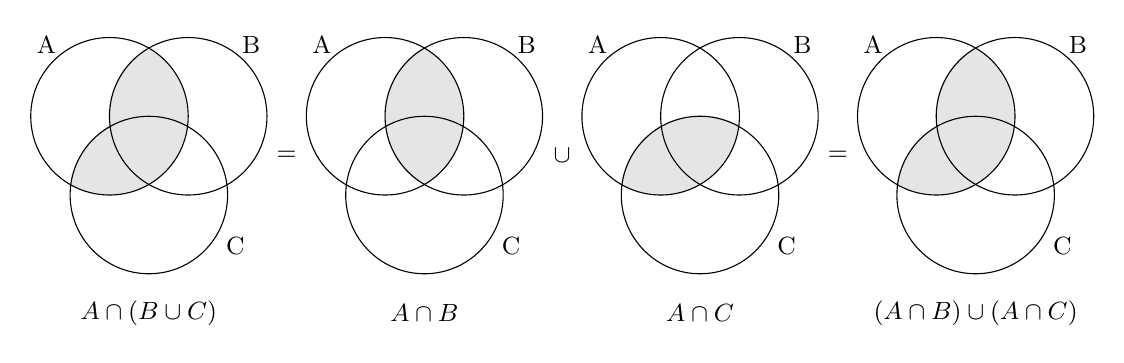
\begin{tikzpicture}[x=5mm, y=5mm,font=\small,filled/.style={fill=circle area, draw=circle edge, thick}]
\def\firstcircle{(0,0) circle (2)}
\def\secondcircle{(2,0) circle (2)}
\def\thirdcircle{(1,-2) circle (2)}

\definecolor{circle edge}{gray}{0.9}
\definecolor{circle area}{gray}{0.9}

   \begin{scope}
        \clip \firstcircle;
        \fill[filled] \secondcircle;
        \fill[filled] \thirdcircle;
    \end{scope}

\draw (0,0) circle (2);
\draw (2,0) circle (2);
\draw (1,-2) circle (2);
\node  at (-1.6,1.8) {A};
\node  at (3.6,1.8) {B};
\node  at (3.2,-3.3) {C};

\begin{scope}[xshift=35mm]
   \begin{scope}
        \clip \firstcircle;
        \fill[filled] \secondcircle;
    \end{scope}
\node  at (-1.6,1.8) {A};
\node  at (3.6,1.8) {B};
\node  at (3.2,-3.3) {C};
\draw (0,0) circle (2);
\draw (2,0) circle (2);
\draw (1,-2) circle (2);
\end{scope}

\begin{scope}[xshift=70mm]
   \begin{scope}
        \clip \firstcircle;
        \fill[filled] \thirdcircle;
    \end{scope}
\node  at (-1.6,1.8) {A};
\node  at (3.6,1.8) {B};
\node  at (3.2,-3.3) {C};
\draw (0,0) circle (2);
\draw (2,0) circle (2);
\draw (1,-2) circle (2);
\end{scope}

\begin{scope}[xshift=105mm]
   \begin{scope}
        \clip \firstcircle;
        \fill[filled] \secondcircle;
        \fill[filled] \thirdcircle;
    \end{scope}
\node  at (-1.6,1.8) {A};
\node  at (3.6,1.8) {B};
\node  at (3.2,-3.3) {C};
\draw (0,0) circle (2);
\draw (2,0) circle (2);
\draw (1,-2) circle (2);
\end{scope}

\foreach \x/\xtext in {4.5/=,11.5/\cup,18.5/=}
\node  at (\x,-1) {$\xtext$};

\foreach \xi/\xitext in {1/$A\cap(B\cup C)$,8/$A\cap B$,15/$A\cap C$,22/$(A\cap B)\cup(A\cap C)$}
\node  at (\xi,-5) {\xitext};
\end{tikzpicture}

\end{center}
% \end{esempio}
%\end{exrig}

\ovalbox{\risolvii \ref{ese:5.56}, \ref{ese:5.57}, \ref{ese:5.58}, \ref{ese:5.59}}

\section{Insieme differenza}

Consideriamo gli insiemi~$A$ e~$B$ formati rispettivamente
dalle lettere dell'alfabeto italiano e dalle
consonanti dell'alfabeto italiano cioè:
$A=\{$a, b, c, d, e, f, g, h, i, l, m, n, o, p, q, r, s, t, u, v, z$\}$ e
$B=\{$b, c, d, f, g, h, l, m, n, p, q, r, s, t, v, z$\}$, le lettere ``a, e, i, o, u'' che compaiono
nell'insieme~$A$ ma non in~$B$ formano un nuovo insieme chiamato insieme \emph{differenza} tra $A$ e $B$.

\begin{definizione}
 Dati due insiemi~$A$ e~$B$, si dice \emph{insieme differenza} tra $A$ e $B$ l'insieme~$C$ composto da tutti gli elementi
di~$A$ che non appartengono a~$B$. In simboli:~$C=A-B$ o anche $C=A \backslash B$.
\end{definizione}

\begin{center}
\input{./lbr/chap05/fig013_dif.pgf}
\end{center}
Mediante proprietà caratteristica si scrive:~$C=A-B=\{x\mid (x\in A)\text{ e }(x\notin B)\}$.

\subsection{Proprietà della differenza tra insiemi}

\begin{enumeratea}
\item $A-A=\emptyset$;
\item $A-\emptyset =A$;
\item se~$A\cap B=\emptyset $, ossia $A$ e $B$ sono disgiunti, allora~$A-B=A$, e~$B-A=B$;
\item se~$B\subset A$, ossia~$B$ è sottoinsieme proprio di~$A$, allora~$B-A=\emptyset $.
\end{enumeratea}

\begin{exrig}
 \begin{esempio}
Siano~$A=\{$ 8, 9, 10, 12, 13$\}$ e~$B=\{$9, 10, 11, 13$\}$, allora
$C=A-B=\{$8, 12$\}$ e~$D=B-A=\{11\}$.
 \end{esempio}
\end{exrig}

Poiché in genere $A-B\neq B-A$, nella differenza tra insiemi non vale la proprietà
commutativa.

\begin{exrig}
 \begin{esempio}
Siano~$D=\{$1, 3, 5$\}$ e~$P=\{$0, 2, 4$\}$. I due insiemi sono disgiunti poiché ~$P\cap D=\emptyset$,
 quindi~$D-P=\{$1, 3, 5$\}=D$ e~$P-D=\{$0, 2, 4$\}=P$.
\begin{center}
 \input{./lbr/chap05/fig014_difi.pgf}
\end{center}
 \end{esempio}
\pagebreak
 \begin{esempio}
Siano~$X=\{$do, re, mi, fa, sol, la, si$\}$
e~$Y=\{$do, re, mi$\}$ allora poiché
$Y\subset X$, $W=X-Y=\{$fa, sol, la, si$\}$.
\begin{center}
 \input{./lbr/chap05/fig015_difii.pgf}
\end{center}
 \end{esempio}
\end{exrig}

\ovalbox{\risolvii \ref{ese:5.60}, \ref{ese:5.61}, \ref{ese:5.62}}

\section{Insieme complementare}

Sia~$W=\{\text{sabato, domenica}\}$ l'insieme dei giorni della settimana che non finiscono per ``dì''.
L'insieme~$W$ può essere considerato come sottoinsieme dell'insieme~$G$ formato da tutti i giorni della settimana
$G=\{\text{lunedì, martedì, mercoledì, giovedì, venerdì, sabato, domenica}\}$.
L'insieme degli elementi di~$G$ che non appartengono a~$W$ forma
un insieme che chiameremo \emph{complementare} di~$W$ rispetto a~$G$. L'insieme~$G$ invece si dice, in questo caso, insieme \emph{universo}. Ad esempio
nella rappresentazione caratteristica~$A=\{x\in\insN\mid x\le~100\}$,
$\insN$ è l'insieme universo di~$A$.

\begin{definizione}
Dato un insieme~$A$, uno dei possibili insiemi che
contengono~$A$ come sottoinsieme si dice
\emph{insieme universo} o \emph{insieme ambiente}.
\end{definizione}

\begin{definizione}
Dato l'insieme~$A$ e scelto~$U$ come suo insieme universo, l'insieme degli elementi di
$U$ che non appartengono ad~$A$ è detto \emph{insieme complementare} di~$A$ rispetto a~$U$ e si indica con~$\overline{A}$ oppure~$\overline{A}_{U}$
o ancora~$\complement_{U}A$.
\end{definizione}

\begin{multicols}{2}
Il diagramma di Eulero-Venn dell'insieme $A$ e del suo universo $U$ è quello rappresentato in figura.
La parte in grigio è il complementare di~$A$ rispetto a~$U$, cioè~${\overline{A}}_{U}$.
Si può osservare che, essendo~$A\subseteq U$, il complementare coincide con la differenza tra insiemi:
${\overline{A}}_{U}=U-A$.
\begin{center}
\input{./lbr/chap05/fig016_com.pgf}
\end{center}
\end{multicols}

\begin{exrig}
 \begin{esempio}
 Insiemi complementari.
\begin{enumeratea}
\item Il complementare dell'insieme~$D$ dei numeri dispari rispetto all'insieme~$\insN$ dei numeri naturali è
l'insieme~$P$ dei numeri pari:~${\overline{D}}_{\insN}=P$;
\item Il complementare dell'insieme~$V$ delle vocali dell'alfabeto italiano rispetto
all'insieme~$A$ delle lettere dell'alfabeto italiano è l'insieme~$C$ delle consonanti:
${\overline{V}}_{U}=C$;
\item Dati gli insiemi~$U=\{x\in \insN\mid 1\le x\le~10\}$ e~$B=\{x\in \insN\mid 1\le x\le~5\}$, poiché $B\subset U$
si può determinare~${\overline{B}}_{U}=\{x\in \insN\mid 6\le x\le~10\}$.
\end{enumeratea}
 \end{esempio}
\end{exrig}

\ovalbox{\risolvii \ref{ese:5.63}, \ref{ese:5.64}, \ref{ese:5.65}, \ref{ese:5.66}}

\section{Leggi di De Morgan}

Dati due insiemi~$A$ e~$B$ ci sono alcune proprietà,
dette \emph{leggi di De Morgan}\footnote{dal nome del matematico e logico britannico Augustus De Morgan (1806 - 1871).}, che semplificano lo svolgimento di alcune operazioni:

\begin{enumeratea}
\item $\overline{A\cap B}=\overline{A}\cup \overline{B}$: \emph{Prima legge di De Morgan};
\item $\overline{A\cup B}=\overline{A}\cap \overline{B}$: \emph{Seconda legge di De Morgan}.
\end{enumeratea}

Dimostriamo la prima legge di De Morgan utilizzando i diagrammi di Eulero-Venn.
\begin{center}
 \input{./lbr/chap05/fig017_dem.pgf}
\end{center}

\ovalbox{\risolvi \ref{ese:5.67}}

\section{Partizione di un insieme}
\begin{definizione}
Dato un insieme~$A$ e alcuni suoi sottoinsiemi $A_1$, $A_2$, $A_3$, \ldots, $A_n$, si dice che questi costituiscono una \emph{partizione} di~$A$ se:
\begin{enumeratea}
 \item sono tutti non vuoti;
 \item sono a due a due disgiunti;
 \item la loro unione dà l'insieme~$A$.
\end{enumeratea}
\end{definizione}

\begin{exrig}
 \begin{esempio}
 Partizione di un insieme.

Dato l'insieme~$C$ delle carte da gioco napoletane, i sottoinsiemi~$C_1$ delle carte a denari, $C_2$ delle carte a spade, $C_3$ delle carte a coppe, $C_4$ delle carte a bastoni costituiscono una partizione di~$C$.

Infatti nessuno degli insiemi $C_1$, $C_2$, $C_3$, $C_4$ è vuoto, ciascuno è costituito da~10 elementi. Inoltre i sottoinsiemi sono a due a due disgiunti perché non ci sono carte che appartengono a $C_1 \cap C_2$, $C_1 \cap C_3$, $C_1 \cap C_4$, $C_2 \cap C_3$, $C_2 \cap C_4$, $C_3 \cap C_4$, cioè non ci sono carte che possono appartenere contemporaneamente a due semi distinti. Infine l'unione $C_1\cup C_2 \cup C_3 \cup C_4$ dà l'insieme delle carte~$C$.
 \end{esempio}
\end{exrig}

\ovalbox{\risolvii \ref{ese:5.68}, \ref{ese:5.69}, \ref{ese:5.70}, \ref{ese:5.71}}

\section{Prodotto cartesiano fra insiemi}

Supponiamo che la partita di calcio Lecce~-~Juventus sia terminata~3-2; in questo caso il risultato della partita
non rappresenta un insieme di numeri dato che nella rappresentazione di un insieme scrivere~$\{$3, 2$\}$ e~$\{$2, 3$\}$
 è la stessa cosa. Infatti, se avessimo scritto~2-3 al posto di~3-2 la partita avrebbe avuto un esito
differente. Ci troviamo nel caso di una \emph{coppia ordinata} di numeri.\footnote{si veda anche la sezione~\ref{sect:coordinate_cartesiane} a pagina~\pageref{sect:coordinate_cartesiane}.}

\begin{definizione}
Un insieme di due elementi~$a$ e~$b$
presi in un determinato ordine si dice \emph{coppia ordinata}. Se il primo elemento della coppia è
$a$ e il secondo è~$b$ si scrive:~$(a;b)$.
\end{definizione}

\begin{definizione}
Dati due insiemi~$A$ e~$B$ non vuoti,
l'insieme formato da tutte le coppie ordinate tali che
il primo elemento appartiene ad~$A$ e il secondo a~$B$, si chiama
\emph{prodotto cartesiano} di~$A$ per~$B$. In simboli:~$A\times B$ che si legge ``$A$ per~$B$''
oppure ``$A$ prodotto cartesiano con~$B$'' o ancora ``$A$ cartesiano~$B$''.
\end{definizione}

Mediante proprietà caratteristica si scrive:
$A\times B=\{(x;y)\mid x\in A\text{ e }y\in B\}$.

Nel caso in cui~$B=A$, il prodotto cartesiano diventa $A\times A=A^{2}=\{(x;y)\mid x\in A\text{ e }y\in A\}$.

\begin{exrig}
 \begin{esempio}
Sia~$C=\{x\text{, }y\text{, }z\}$, il prodotto cartesiano~$C\times C$ è dato dalle
seguenti coppie ordinate:~$C\times C=\{(x;x)\text{, }(x;y)\text{, }(x;z)\text{, }(y;x)\text{, }(y;y)\text{, }(y;z)\text{, }(z;x)\text{, }(z;y)\text{, }(z;z)\}$.
 \end{esempio}
\end{exrig}

\subsection{Proprietà del prodotto cartesiano tra insiemi}
\begin{multicols}{3}
\begin{enumeratea}
 \item $A\times \emptyset =\emptyset$;
 \item $\emptyset \times A=\emptyset$;
 \item $\emptyset \times \emptyset =\emptyset$.
\end{enumeratea}
\end{multicols}

\begin{exrig}
 \begin{esempio}
Sia~$A=\{\text{a, b}\}$ e~$B=\{\text{1, 2, 3}\}$. Il prodotto cartesiano~$A\times B$ è dato dalle seguenti coppie ordinate:
$A\times B=\{(\text{a};1)\text{, }(\text{a};2)\text{, }(\text{a};3)\text{, }(\text{b};1)\text{, }(\text{b};2)\text{, }(\text{b};3)\}$, mentre il prodotto cartesiano~$B\times A$
è dato dalle seguenti coppie ordinate:
$B\times A=\{(1;\text{a})\text{, }(2;\text{a})\text{, }(3;\text{a})\text{, }(1;\text{b})\text{, }(2;\text{b})\text{, }(3;\text{b})\}$.
Quindi si può notare che~$A\times B\neq B\times A$.
 \end{esempio}
\end{exrig}

Poiché $A\times B\neq B\times A$ nel prodotto cartesiano non vale la
proprietà commutativa.

\vspazio\ovalbox{\risolvii \ref{ese:5.72}, \ref{ese:5.73}, \ref{ese:5.74}, \ref{ese:5.75}, \ref{ese:5.76}, \ref{ese:5.77}}

\subsection{Rappresentazione del prodotto cartesiano tra insiemi}
\paragraph{Tabulazione delle coppie ordinate}

Come fatto nei precedenti esempi, si combina il primo elemento
di~$A$ con tutti gli elementi di~$B$, il secondo elemento
di~$A$ con tutti gli elementi di~$B$ e cosi via fino ad
esaurire tutti gli elementi di~$A$.
\[A\times B=\{(\text{a};1)\text{, }(\text{a};2)\text{, }(\text{a};3)\text{, }(\text{b};1)\text{, }(\text{b};2)\text{, }(\text{b};3)\}.\]

\paragraph{Diagramma a frecce}
Si rappresentano i due insiemi graficamente
con i diagrammi di Eulero-Venn e si tracciano degli archi orientati che
escono dagli elementi del primo insieme e raggiungono gli elementi del
secondo insieme formando coppie ordinate del prodotto cartesiano.
\begin{center}
\input{./lbr/chap05/fig019_fre.pgf}
\end{center}

\paragraph{Tabella a doppia entrata}

Si costruisce una tabella nella quale si riportano gli elementi del
primo insieme sulla prima colonna e gli elementi del secondo insieme
sulla prima riga. Le caselle di incrocio rappresentano le coppie
ordinate del prodotto cartesiano.
\begin{center}
 \input{./lbr/chap05/fig020_tab.pgf}
\end{center}

\begin{wrapfloat}{figure}{r}{0pt}
 % (c) 2012 Dimitrios Vrettos - d.vrettos@gmail.com
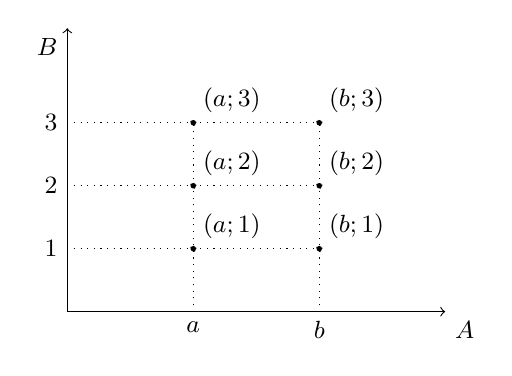
\begin{tikzpicture}[x=16mm, y=8mm,font=\small]
\draw[->] (0,0)--(3,0) node [below right]{$A$};
\draw[->] (0,0)--(0,4.5) node [below left]{$B$};

\begin{scope}[dotted]
\foreach \x in {1,2}
\foreach \y in {1,2,3}{
\draw (\x,0) -- (\x,\y);
\draw (0,\y) -- (\x,\y);
\draw[fill](\x,\y) circle (1pt);
}
\end{scope}

\begin{scope}[above right]
\node at (1,1) {$(\text{a};1)$};
\node at (1,2) {$(\text{a};2)$};
\node at (1,3) {$(\text{a};3)$};
\node at (2,1) {$(\text{b};1)$};
\node at (2,2) {$(\text{b};2)$};
\node at (2,3) {$(\text{b};3)$};
\end{scope}

\foreach \xi/\xitext in {1/$\text{a}$,2/$\text{b}$}
\node[below] at (\xi,0) {\xitext};

\foreach \yi/\yitext in {1/1,2/2,3/3}
\node[left] at (0,\yi) {\yitext};

\end{tikzpicture}

\end{wrapfloat}

\paragraph{Diagramma cartesiano}
Si tracciano due semirette orientate, perpendicolari, una orizzontale e l'altra
verticale, con l'origine
in comune. Si riportano gli elementi del primo insieme sulla semiretta
orizzontale e quelli del secondo su quella verticale. Tali semirette
vengono chiamate \emph{assi cartesiani}. Si tracciano prima le
parallele all'asse verticale dai punti individuati
sull'asse orizzontale che rappresentano gli elementi
del primo insieme, poi le parallele all'asse
orizzontale dai punti sull'asse verticale; i punti di
intersezione rappresentano le coppie ordinate del prodotto
cartesiano.

\paragraph{Diagramma ad albero}
\`E un grafico formato da un nodo iniziale dal quale si ripartono alcuni
rami che a loro volta possono ramificarsi e così via fino a che nello
schema figurano tutte le possibili situazioni.
Si può raggiungere un particolare nodo solo muovendosi lungo i rami ed
il percorso che collega due nodi qualsiasi deve essere unico.

La rappresentazione mediante diagramma ad albero è vantaggiosa nel
caso si voglia fare il prodotto cartesiano tra più insiemi.
\begin{center}
\input{./lbr/chap05/fig022_alb.pgf}
\end{center}

\begin{exrig}
 \begin{esempio}
 Una compagnia aerea deve organizzare delle rotte per collegare fra loro alcune città effettuando uno scalo
in un'altra città. Sia~$P=\{$Brindisi, Bari, Palermo$\}$ l'insieme delle città di
partenza, $S=\{$Roma, Milano$\}$ l'insieme delle città di
scalo e~$A=\{$Parigi, Berlino, Londra$\}$ l'insieme delle città di
arrivo. Per conoscere tutte le possibili rotte aeree dobbiamo
determinare il prodotto cartesiano tra i~3 insiemi~$P\times S\times A$.
Rappresentiamo~$P\times S\times A$ tramite un diagramma ad albero:
%\newpage
\begin{center}
% (c) 2012 Dimitrios Vrettos - d.vrettos@gmail.com
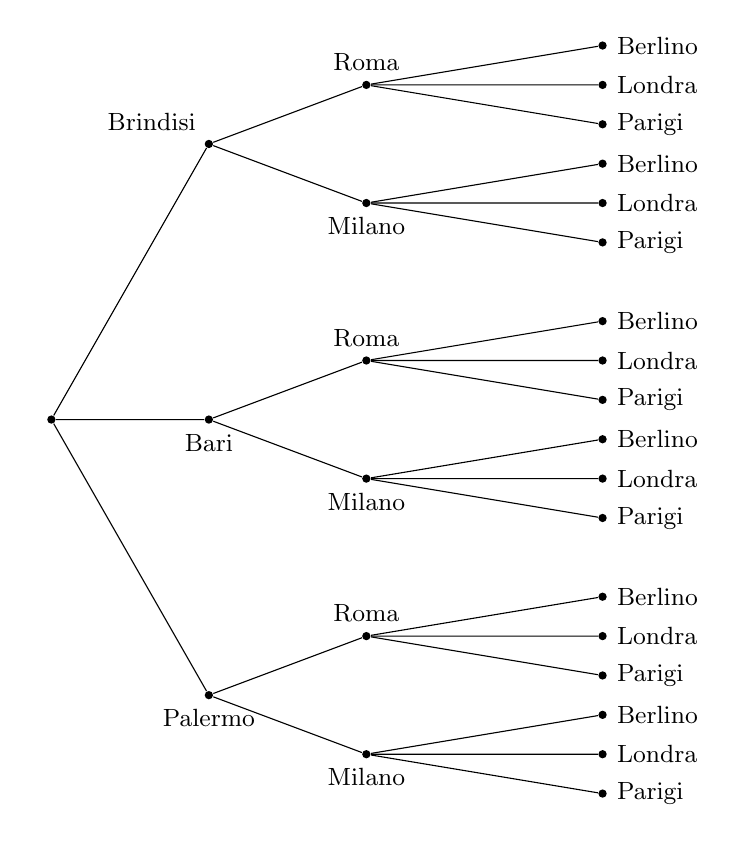
\begin{tikzpicture}[x=5mm, y=5mm,font=\small]
\tikzstyle{level 1}=[level distance=2cm, sibling distance=3.5cm]
\tikzstyle{level 2}=[level distance=2cm, sibling distance=1.5cm]
\tikzstyle{level 3}=[level distance=3cm, sibling distance=.5cm]
\tikzstyle{point} = [circle,minimum width=3pt,fill, inner sep=0pt]

\node[point, label=left:{}] (aer) at (0,0) {}[grow'=right]
  child {node[point, label=above left:{Brindisi}] {} 
    child {node[point,label=above:{Roma}] {}
      child {node[point, label=right:{Berlino}] {}}
      child {node[point, label=right:{Londra}] {}}
      child {node[point, label=right:{Parigi}] {}}
    }
    child {node[point,label=below:{Milano}] {}
      child {node[point, label=right:{Berlino}] {}}
      child {node[point, label=right:{Londra}] {}}
      child {node[point, label=right:{Parigi}] {}}}
    }
  child {node[point, label=below:{Bari}] {} 
    child {node[point,label=above:{Roma}] {}
      child {node[point, label=right:{Berlino}] {}}
      child {node[point, label=right:{Londra}] {}}
      child {node[point, label=right:{Parigi}] {}}}
    child {node[point,label=below:{Milano}] {}
      child {node[point, label=right:{Berlino}] {}}
      child {node[point, label=right:{Londra}] {}}
      child {node[point, label=right:{Parigi}] {}}}
    }
  child {node[point, label=below:{Palermo}] {} 
    child {node[point,label=above:{Roma}] {}
      child {node[point, label=right:{Berlino}] {}}
      child {node[point, label=right:{Londra}] {}}
      child {node[point, label=right:{Parigi}] {}}}
    child {node[point,label=below:{Milano}] {}
      child {node[point, label=right:{Berlino}] {}}
      child {node[point, label=right:{Londra}] {}}
      child {node[point, label=right:{Parigi}] {}}}
};
\end{tikzpicture}

\end{center}
 \end{esempio}
\end{exrig}

\section{I diagrammi di Eulero-Venn come modello di un problema}
Alcune volte, trovandoci di fronte a un problema, possiamo rappresentare
la situazione con diagrammi di Eulero-Venn, ciò agevola la
comprensione e facilita la risoluzione del problema. Attraverso alcuni
esempi mostreremo come usare la teoria degli insiemi per risolvere
problemi.

\begin{exrig}
 \begin{esempio}
Nel seguente diagramma di Eulero-Venn, l'insieme~$A$ rappresenta un gruppo di amici appassionati di ballo; gli insiemi~$T$, $R$,
$S$ rappresentano rispettivamente coloro che ballano il tango, la rumba, il samba; ogni puntino rappresenta uno degli amici.
\begin{multicols}{2}
Quanti sono gli amici appassionati di ballo?

Quanti tra loro ballano:
\begin{enumeratea}
\item \emph{nessuno} dei balli indicati?
\item \emph{almeno uno} dei balli tango, samba, rumba?
\item \emph{almeno} il samba?
\item \emph{solo} la rumba?
\item la rumba \emph{e} il tango?
\item \emph{tutti} i balli indicati?
\end{enumeratea}
\begin{center}
 % (c) 2012 Dimitrios Vrettos - d.vrettos@gmail.com
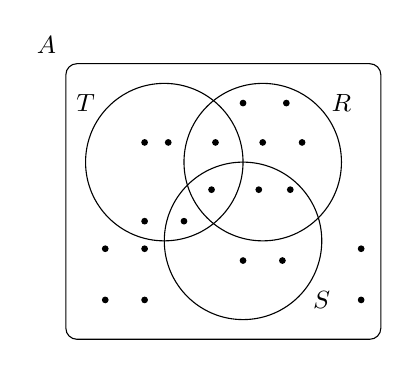
\begin{tikzpicture}[x=5mm, y=5mm,font=\small]

\draw[rounded corners] (0,0) rectangle (8,7) (0,7) node [above left]  {$A$};
\draw (2.5,4.5) circle (2) (.5,6)node {$T$};
\draw (5,4.5) circle (2) (7,6)node {$R$};
\draw (4.5,2.5) circle (2) (6.5,1)node {$S$};

\foreach \x in {2,2.6,3.8,5,6}
\draw[fill] (\x,5) circle (1pt);

\foreach \xi in {4.5,5.6}
\draw[fill] (\xi,6) circle (1pt);

\foreach \xii in {3.7,4.9,5.7}
\draw[fill] (\xii,3.8) circle (1pt);

\foreach \xiii in {2,3}
\draw[fill] (\xiii,3) circle (1pt);

\foreach \xiv in {4.5,5.5}
\draw[fill] (\xiv,2) circle (1pt);

\foreach \xv in {1,2,7.5}{
\draw[fill] (\xv,1) circle (1pt);
\draw[fill] (\xv,2.3) circle (1pt);
}
\end{tikzpicture}

\end{center}
\end{multicols}

Per rispondere alle domande dobbiamo contare gli elementi che formano determinati insiemi.

Quanti sono gli amici appassionati di ballo? Per rispondere a questa
domanda, contiamo tutti i puntini che compaiono nel disegno. Si ha 
$\card(A)=20$.

Rispondiamo ora alle altre domande.
\begin{enumeratea}
\item Quanti tra loro ballano \emph{nessuno} dei balli indicati?
Chi non balla nessuno dei balli indicati sta nell'insieme~$A$, ma in nessuno degli insiemi
$R$, $S$, $T$ quindi appartiene al complementare
di~$R\cup S\cup T$ rispetto all'insieme~$A$,
dunque~$\card(\overline{({R\cup S\cup T})}_{A})=6$.

\item Quanti tra loro ballano \emph{almeno uno} dei balli tra tango, samba, rumba? Chi balla almeno uno di quei balli è rappresentato dagli elementi
dell'insieme~$R\cup S\cup T$, quindi~$\card(R\cup S\cup T)=14$.

\item Quanti tra loro ballano \emph{almeno} il samba?
Gli amici che ballano almeno il samba sono nell'insieme
$S$, quindi~$\card(S)=6$.

\item Quanti tra loro ballano \emph{solo} la rumba? Nell'insieme~$R$ sono rappresentati gli amici che
ballano almeno il rumba, quindi dobbiamo togliere dall'insieme~$R$ gli elementi che stanno in
$S$ o in~$T$:~$\card(R-(T\cup S))=4$.

\item Quanti tra loro ballano la rumba \emph{e} il tango? Quelli che ballano sia la rumba che il tango sono gli elementi
dell'insieme intersezione~$R\cap T$, quindi~$\card(R\cap T)=2$.

\item Quanti tra loro ballano \emph{tutti} i balli indicati? Quelli che ballano tutti e tre i balli indicati sono elementi
dell'insieme intersezione~$R\cap S\cap T$, quindi~$\card(R\cap S\cap T)=1$.
\end{enumeratea}
 \end{esempio}

 \begin{esempio}
 A settembre, per la festa delle contrade, a Lainate è arrivato un luna
park dove, oltre ad una grande giostra, era stato allestito un tiro a
segno con palline di gommapiuma, proprio per i bambini. Alcuni
bambini, accompagnati dalla loro maestra si sono recati al luna park: 7
sono stati sulla giostra, 3 sono stati sia sulla giostra che al tiro a
segno, 3 si sono divertiti solamente col tiro a segno e altri~2 sono
stati a guardare. Quanti bambini sono andati quel giorno al luna park?

\begin{multicols}{2}
Per risolvere il problema rappresentiamo con diagrammi di Eulero-Venn la situazione; indichiamo con~$B$ l'insieme dei
bambini recatisi al luna park, con~$G$ l'insieme di quelli che sono stati sulla giostra e con~$T$ l'insieme
di quelli che hanno provato il tiro a segno.
Dall'enunciato sappiamo che~$\card(G)=7$, $\card(G\cap T)=3$, $\card(T-G)=3$ e~$\card(B-(G\cup T))=2$.
\begin{center}
 \input{./lbr/chap05/fig025_evi.pgf}
\end{center}
\end{multicols}

Completa la rappresentazione segnando i bambini con dei puntini e rispondi al quesito.
\end{esempio}

\begin{esempio}
Alla palestra Anni Verdi, il giovedì si tengono due allenamenti di pallavolo e calcio dalle~17.00 alle~18.30. Frequentano il corso di
pallavolo~15 persone e sono~28 quelli che frequentano l'allenamento di calcio. Quante persone frequentano
pallavolo o calcio in questo orario?
\paragraph{Dati} $P=\{$iscritti a pallavolo$\}$, $C=\{$iscritti a calcio$\}$, $\card(P)=15$, $\card(C)=28$.
\paragraph{Obiettivo} Il problema chiede di determinare la cardinalità di~$P\cup C$.
%\begin{multicols}{2}
\paragraph{Soluzione} Osserviamo che non ci sono persone che frequentano sia
l'uno che l'altro sport essendo gli allenamenti nello stesso orario; gli insiemi~$P$ e~$C$
sono disgiunti:~$P\cap C=\emptyset $. Quindi:~$\card(P\cup C)=\card(P)+\card(C)=15+28=43$.
\end{esempio}

\begin{esempio}
\begin{multicols}{2}
 Alla palestra Anni Verdi, il lunedì si tengono allenamenti di pallavolo dalle~17.00 alle~18.30 e dalle~19.00 alle~20.30 gli
allenamenti di calcio. Quelli che frequentano la pallavolo sono~15, quelli che frequentano il calcio sono~28, però ce ne sono~7 di loro
che fanno entrambi gli allenamenti. Quanti sono gli sportivi che si allenano il lunedì?
\begin{center}
 % (c) 2012 Dimitrios Vrettos - d.vrettos@gmail.com
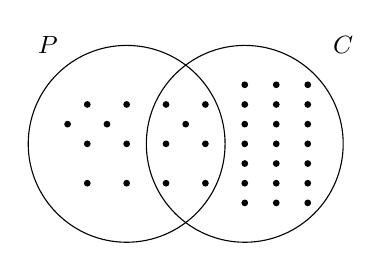
\begin{tikzpicture}[x=5mm, y=5mm,font=\small]

\draw (2,0) circle (2.5) (0,2.5)node {$P$};
\draw (5,0) circle (2.5) (7.5,2.5)node {$C$};

\foreach \x in {1,2,3,4}
\foreach \y in {-1,0,1}
\draw[fill] (\x,\y) circle (1pt);

\foreach \z in {.5,1.5,3.5}
\draw[fill] (\z,.5) circle (1pt);

\foreach \i in {5,5.8,6.6}
\foreach \j in {1.5,1,.5,0,-.5,-1,-1.5}
\draw[fill] (\i,\j) circle (1pt); 
\end{tikzpicture}

 \end{center}
\end{multicols}
\paragraph{Dati} $P=\{$iscritti a pallavolo$\}$, $C=\{$iscritti a calcio$\}$, $\card(P)=15$, $\card(C)=28$ e~$\card(P\cap C)=7$.\paragraph{Obiettivo} Il problema chiede di determinare la cardinalità di~$P\cup C$.
\paragraph{Soluzione} Poiché gli insiemi $P$ e $C$ non sono disgiunti, si ha $\card(P\cup C)=\card(P)+\card(C)-\card(P\cap C)=15+28-7=36$.

Generalizzando possiamo affermare che, dati due insiemi finiti~$A$ e~$B$, la cardinalità dell'insieme~$A\cup B$ è data dalla seguente formula:
\[\card(A\cup B)=\card(A)+\card(B)-\card(A\cap B).\]
\end{esempio}

\begin{esempio}
 A scuola si sono aperti i corsi di lingue. Della classe di Piero, che è composta da~28 ragazzi, 17 frequentano il corso di inglese, 12
quello di francese, 5 di loro frequentano sia il corso di inglese che quello di francese. Quanti sono i ragazzi della classe di Piero che non
frequentano alcun corso di lingue?

Rappresentiamo la situazione con un diagramma di Eulero-Venn.
\begin{multicols}{2}
L'insieme universo è costituito dai~28 ragazzi che
compongono la classe. I ragazzi che frequentano almeno un corso non sono~$17+12=29$, perché ce ne sono~5 che frequentano entrambi i corsi e così
vengono conteggiati due volte. Quindi i ragazzi che frequentano almeno un corso sono~$17+12-5=24$. Di conseguenza quelli che non frequentano
nessun corso sono~$28-24=4$.
\begin{center}
 \input{./lbr/chap05/fig027_eviii.pgf}
\end{center}
\end{multicols}
\end{esempio}

\begin{esempio}
 Il professore di matematica di Piero è piuttosto severo; nella sua classe, di~28 alunni, ha messo solo~6 sufficienze allo scritto e solo~8
all'orale. I ragazzi che sono risultati insufficienti sia allo scritto sia all'orale sono stati~18. Quanti
sono i ragazzi che hanno avuto una votazione sufficiente sia allo scritto che all'orale?

Rappresentiamo la situazione con un diagramma di Eulero-Venn.
\begin{multicols}{2}
$C$ è l'insieme degli alunni della classe di Piero ed è costituito da~28 elementi. $S$ è l'insieme dei ragazzi
sufficienti allo scritto costituito da~6 alunni. $O$ è l'insieme dei ragazzi che sono sufficienti
all'orale ed è costituito da~8 elementi.

Gli elementi di~$\overline{S\cup O}$ sono~18, cioè i ragazzi che
non sono sufficienti né allo scritto, né all'orale.
\begin{center}
 \input{./lbr/chap05/fig028_eviv.pgf}
\end{center}
\end{multicols}

L'insieme~$S\cup O$ è quindi costituito da~$28-18=10$ elementi.

Ricordiamo che
\begin{align*}
 &\card(S\cup O)=\card(S)+\card(O)-\card(S\cap O)\\
 \Rightarrow &\card(S\cap O)=\card(S)+\card(O)-\card(S\cup O)\\
 \Rightarrow &\card(S\cap O)=6+8-10=4.
\end{align*}
In conclusione i ragazzi sufficienti allo scritto e all'orale sono~4.
\end{esempio}
\end{exrig}

\ovalbox{\risolvii \ref{ese:5.78}, \ref{ese:5.79}, \ref{ese:5.80}, \ref{ese:5.81}, \ref{ese:5.82}, \ref{ese:5.83}, \ref{ese:5.84}, \ref{ese:5.85}, \ref{ese:5.86}, \ref{ese:5.87},
\ref{ese:5.88}, \ref{ese:5.89}, \ref{ese:5.90}}

\vspazio\ovalbox{\ref{ese:5.91}}

\newpage
% (c) 2012 Dimitrios Vrettos - d.vrettos@gmail.com
% (c) 2012 Claudio Carboncini - claudio.carboncini@gmail.com
\section{Esercizi}
\subsection{Esercizi dei singoli paragrafi}
\subsubsection*{\thechapter.1 - Insiemi ed elementi}

\begin{esercizio}
 \label{ese:5.1}
 Barra con una crocetta i raggruppamenti che ritieni siano degli insiemi.
 \begin{multicols}{2}
 \begin{enumeratea}
\item I fiumi più lunghi d'Italia;
\item le persone con più di~30 anni;
\item i numeri~1, 20, 39, 43, 52;
\item i libri più pesanti nella tua cartella;
\item i punti di una retta;
\item gli animali con~2 zampe;
\item le vocali dell'alfabeto italiano;
\item i professori bravi;
\item i gatti con due code;
\item i calciatori che hanno fatto pochi gol.
\end{enumeratea}
\end{multicols}
\end{esercizio}

%%%%%%%%%%%%%%%%%%%%%%%%%%%%%%%%%%%%%%%%%%%%%%%%%%%%%%%%%%%%%%%%%%%%%
\begin{esercizio}
 \label{ese:5.2}
Considerando l'insieme $A$ delle lettere dell'alfabeto italiano, per ciascuno dei seguenti casi inserisci il simbolo adatto fra ``$\in$'' e ``$\notin$''.

b \ldots $A$, i \ldots $A$, j \ldots $A$, e \ldots $A$, w \ldots $A$, z \ldots $A$.
\end{esercizio}

\begin{esercizio}
\label{ese:5.3}
Le vocali delle parole che seguono formano insiemi uguali, tranne in un caso. Quale?
\begin{center}
 \boxA\quad sito\quad\boxB\quad micio\quad\boxC\quad zitto\quad\boxD\quad fiocco\quad\boxE\quad lecito\quad\boxF\quad dito.
\end{center}
\end{esercizio}

\begin{esercizio}
\label{ese:5.4}
Individua tra i seguenti insiemi quelli che sono uguali:
\begin{multicols}{2}
\begin{enumeratea}
 \item vocali della parola ``SASSO'';
 \item consonanti della parola ``SASSO'';
 \item vocali della parola ``PIETRA'';
 \item vocali della parola ``PASSO''.
\end{enumeratea}
\end{multicols}
\end{esercizio}

\begin{esercizio}
\label{ese:5.5}
Quali delle seguenti frasi rappresentano criteri oggettivi per individuare un insieme? Spiega perché.
\TabPositions{8.5cm}
\begin{enumeratea}
\item Le città che distano meno di~100 km da Lecce; \tab\boxV\quad\boxF
\item i laghi d'Italia;  \tab\boxV\quad\boxF
\item le città vicine a Roma; \tab\boxV\quad\boxF
\item i calciatori della Juventus;  \tab\boxV\quad\boxF
\item i libri di Mauro;  \tab\boxV\quad\boxF
\item i professori bassi della tua scuola;  \tab\boxV\quad\boxF
\item i tuoi compagni di scuola il cui nome inizia per M; \tab\boxV\quad\boxF
\item i tuoi compagni di classe che sono gentili; \tab\boxV\quad\boxF
\item gli zaini neri della tua classe.  \tab\boxV\quad\boxF
\end{enumeratea}
\end{esercizio}

\begin{esercizio}
\label{ese:5.6}
Scrivi al posto dei puntini il simbolo mancante tra ``$\in$'' e ``$\notin$''.

\begin{enumeratea}
\item La Polo \ldots\ldots all'insieme delle automobili Fiat;
\item il cane \ldots\ldots all'insieme degli animali domestici;
\item la Puglia \ldots\ldots all'insieme delle regioni italiane;
\item Firenze \ldots\ldots all'insieme delle città francesi;
\item il numero~10 \ldots\ldots all'insieme dei numeri naturali;
\item il numero~3 \ldots\ldots all'insieme dei numeri pari.
\end{enumeratea}
\end{esercizio}
\pagebreak
\begin{esercizio}
\label{ese:5.7}
Quali delle seguenti proprietà sono caratteristiche per un insieme?
\TabPositions{8.5cm}
\begin{enumeratea}
\item Essere una città italiana il cui nome inizia per W; \tab\boxV\quad\boxF
\item essere un bravo cantante; \tab\boxV\quad\boxF
\item essere un monte delle Alpi;  \tab\boxV\quad\boxF
\item essere un ragazzo felice; \tab\boxV\quad\boxF
\item essere un numero naturale grande;\tab\boxV\quad\boxF
\item essere un ragazzo nato nel~1985; \tab\boxV\quad\boxF
\item essere un alunno della classe~1\textsuperscript{a}C; \tab\boxV\quad\boxF
\item essere una lettera dell'alfabeto inglese; \tab\boxV\quad\boxF
\item essere una retta del piano; \tab\boxV\quad\boxF
\item essere un libro interessante della biblioteca; \tab\boxV\quad\boxF
\item essere un italiano vivente nato nel~1850; \tab\boxV\quad\boxF
\item essere un italiano colto. \tab\boxV\quad\boxF
\end{enumeratea}
\end{esercizio}

\begin{esercizio}
\label{ese:5.8}
Scrivi al posto dei puntini il simbolo mancante tra ``$=$'' e ``${\neq}$''.
\begin{enumeratea}
\item L'insieme delle lettere della parola ``CANE'' e della parola ``PANE'' sono \ldots\ldots;
\item l'insieme delle vocali della parola ``INSIEME'' e della parola ``MIELE'' sono \ldots\ldots;
\item l'insieme delle consonanti della parola ``LETTO'' e della parola ``TETTO'' sono \ldots\ldots;
\item l'insieme delle lettere della parola ``CONTRO'' e della parola ``TRONCO'' sono \ldots\ldots;
\item l'insieme delle vocali della parola ``LIBRO'' e della parola ``MINISTRO'' sono \ldots\ldots;
\item l'insieme delle vocali della parola ``DIARIO'' e della parola ``RAMO'' sono \ldots\ldots;
\item l'insieme delle lettere della parola ``MOUSE'' e della parola ``MUSEO'' sono \ldots\ldots;
\item l'insieme delle consonanti della parola ``SEDIA'' e della parola ``ADESSO'' sono \ldots\ldots;
\item l'insieme dei numeri pari minori di~5 e l'insieme vuoto sono \ldots\ldots;
\item l'insieme dei numeri pari e l'insieme dei multipli di~2 sono \ldots\ldots
\end{enumeratea}
\end{esercizio}

\begin{esercizio}
\label{ese:5.9}
Le stelle dell'universo formano un insieme. Le stelle visibili a occhio nudo formano un insieme? Spiega il tuo punto di vista.
\end{esercizio}

\subsubsection*{\thechapter.2 - Insieme vuoto, insieme universo, cardinalità}
\begin{esercizio}
\label{ese:5.10}
Indica se gli insiemi~$G =\{\text{gatti con~6 zampe}\}$ e~$P = \{\text{polli con~2 zampe}\}$ sono o non sono vuoti.
\end{esercizio}

\begin{esercizio}
\label{ese:5.11}
Barra con una croce gli insiemi vuoti.
\begin{enumeratea}
 \item L'insieme dei numeri positivi minori di~0;
 \item l'insieme dei numeri negativi minori di~100;
 \item l'insieme dei numeri pari minori di~100;
 \item l'insieme delle capitali europee della regione Lombardia;
 \item l'insieme dei triangoli con quattro angoli;
 \item l'insieme delle capitali italiane del Lazio;
 \item l'insieme dei punti di intersezione di due rette parallele.
 \end{enumeratea}
\end{esercizio}

\begin{esercizio}
\label{ese:5.12}
Quali delle seguenti scritture sono corrette per indicare
l'insieme vuoto?
\begin{center}
 \boxA\quad~$\emptyset $ \quad\boxB\quad~0 \quad\boxC\quad~$\{\emptyset \}$ \quad\boxD\quad~$\{0\}$ \quad\boxE\quad \{ \}.
\end{center}
\end{esercizio}
\pagebreak
\begin{esercizio}
\label{ese:5.13}
Quali dei seguenti insiemi sono vuoti? Per gli insiemi non vuoti indica la cardinalità.
\begin{enumeratea}
\item L'insieme degli uccelli con~6 ali;
\item l'insieme delle lettere della parola ``VOLPE'';
\item l'insieme dei cani con~5 zampe;
\item l'insieme delle vocali della parola ``COCCODRILLO'';
\item l'insieme delle vocali dell'alfabeto italiano;
\item l'insieme degli abitanti della luna;
\item l'insieme dei numeri sulla tastiera del telefonino.
\end{enumeratea}
\end{esercizio}

\begin{esercizio}
\label{ese:5.14}
Scrivi per ciascun insieme un possibile insieme universo.
\begin{enumeratea}
\item l'insieme dei rettangoli;
\item l'insieme dei multipli di~3;
\item l'insieme delle lettere della parola ``MATEMATICA'';
\item l'insieme dei libri di matematica;
\item l'insieme dei ragazzi che hanno avuto un'insufficienza in matematica.
\end{enumeratea}
\end{esercizio}

\begin{esercizio}
\label{ese:5.15}
Dato l'insieme~$A = \{\text{0, 2, 5}\}$ determina se le seguenti affermazioni sono vere o false.
\TabPositions{2.5cm}
\begin{enumeratea}
\item $0\in A$. \tab\boxV\quad\boxF
\item $5\in A$. \tab\boxV\quad\boxF
\item $\emptyset \in A$. \tab\boxV\quad\boxF
\item $A\in A$. \tab\boxV\quad\boxF
\item $\np{3,5}\in A$. \tab\boxV\quad\boxF
\end{enumeratea}
\end{esercizio}

\cleardoublepage
